%!TeX root = thesis-main.tex
%basicstyle=\fontsize{8}{9}\selectfont\ttfamily

%%%%%%% %%%%%%%%  %%%%%%% 
%%%%%%% COMMANDS  %%%%%%%
%%%%%%% %%%%%%%%  %%%%%%%


\sloppypar

%\chapter{Towards Reinforcement Learning-based Aggregate Computing}
\chapter{Program Sketching with Aggregate Computing}
\minitoc% Creating an actual minitoc
\begin{comment}
The pervasiveness of computing and networking
 fosters applications 
 backed by large-scale cyber-physical collectives---cf. edge-fog-cloud infrastructures, robot swarms, %power grids, 
 and smart ecosystems.
%
Combined with the \emph{autonomic computing} vision ~\cite{DBLP:journals/computer/KephartC03}, which promotes autonomy and self-* capabilities in engineered systems,
 there is an increasing trend towards \acp{cas} and their engineering~\cite{DBLP:journals/sttt/NicolaJW20,DBLP:journals/tasm/BucchiaroneDPCS20}.
%
\acp{cas} are characterized 
 by a multitude of agents  
 that can produce globally coherent results (\emph{emergents}~\cite{DBLP:conf/atal/WolfH04}),
 and collective-level adaptivity to environment change
 via local decision-making and decentralized interaction.
%
The \emph{engineering of \acp{cas}} is an open research problem~\cite{DBLP:journals/sttt/NicolaJW20,DBLP:journals/corr/abs-1108-5643} of significance, tightly linked with the problems of ``steering'' self-organization and ``controlling'' emergence to promote desired while avoiding undesired emergents~\cite{DBLP:books/sp/08/Muller-SchloerS08}.
%
In general, when dealing with \acp{cas},
 there are two distinct problems:
 (i) given an initial system state and local behavioural rules, predicting what global outcomes will be produced (\emph{forward}, \emph{prediction}, or \emph{local-to-global problem});
 and
 (ii) what local behavioural rules must be assigned to the system devices to achieve certain global outcomes (\emph{inverse}, \emph{control}, or \emph{global-to-local problem}).
%
These two problems provide corresponding perspectives
 for \emph{designing} \acp{cas}.
% 
In particular, the latter perspective has promoted research on \emph{spatial} and \emph{macro-programming}~\cite{beal2013organizing-aggregate,DBLP:journals/corr/abs-2201-03473}
 aiming at expressing programs in terms of the desired global outcome
 and leaving the underlying platform to deal with the global-to-local mapping.

In this work,
 we consider \emph{\ac{ac}}~\cite{DBLP:journals/computer/BealPV15}, a prominent \emph{field-based coordination} approach~\cite{DBLP:journals/jlap/ViroliBDACP19} 
promoting macro-programming 
 by capturing \ac{cas} behaviours 
 as functions operating on \emph{computational fields}~\cite{DBLP:journals/jlap/ViroliBDACP19},
 in a system model of neighbour-interacting devices
 operating in asynchronous sense-compute-interact rounds.
%
A computational field is a macro-abstraction
 that maps a set of devices over time to computational values.
%
\ac{ac} is based on the \emph{\ac{fc}}~\cite{DBLP:journals/jlap/ViroliBDACP19}, or variants thereof,
 that define constructs for manipulating and evolving fields.
%
\end{comment}
\ac{cas} behaviour
 can be expressed by a single \emph{aggregate program} (global perspective)
 that also defines 
 what processing and communication activities
 must be performed by each individual device (local perspective).

Besides the programming model and its implications,
 a significant portion of research on \ac{ac}~\cite{DBLP:journals/jlap/ViroliBDACP19} has focussed
 on design and analysis of \emph{coordination algorithms} expressed in \ac{fc}
 for efficiently carrying out self-organising behaviours
 like, e.g., computing fields of minimum distances from sources (\emph{gradients})~\cite{DBLP:conf/ipsn/NagpalSB03,DBLP:journals/pervasive/MameiZL04,DBLP:conf/saso/AudritoCDV17},
 electing leaders~\cite{DBLP:conf/saso/MoBD18},
 or %collecting data %on spanning trees 
 %for 
 distributed summarization~\cite{DBLP:journals/cee/AudritoCDPV21}.
%
However, devising self-organising coordination algorithms is not easy; especially difficult is identifying solutions
 that are efficient across environment assumptions, configurations, and perturbations.
%
The difficulty lies in determining, 
 for a current context,
 the local decisions of each device, 
 in terms e.g. of processing steps and communication acts,
 producing output fields that quickly converge to the correct solution.

In chapter, we start what we consider a key future research thread of field-based coordination, i.e.,
 the study of Machine Learning techniques 
 to improve existing \ac{ac} coordination algorithms.
%
Specifically, we adopt a \emph{\ac{rl}-based approach}---where an agent learns from experience
 how to behave in order to maximize delayed cumulative rewards~\cite{sutton2018reinforcement-learning}.
%
We devise a general methodology that somewhat resembles the notion of \emph{sketching} in program synthesis~\cite{solar2008program-synthesis-sketching}:
 a template program is given and \emph{holes} are filled with actions determined through search.
%
In our case, the program is the \ac{ac} specification of a coordination algorithm, and holes are filled with actions of a policy learnt through Hysteretic Q-Learning~\cite{DBLP:conf/iros/MatignonLF07}.
%
We consider the case of the classic gradient algorithm, a paradigmatic and key building block of self-organising coordination \cite{DBLP:journals/jlap/ViroliBDACP19,beal2013organizing-aggregate,DBLP:journals/corr/abs-2201-03473}: we show via simulations 
 that the system, after sufficient training,
 learns an improved way to compute and adjust gradient fields to network perturbations.

% In the rest of the paper: 
% \Cref{coordination2022:s:background} offers background on \ac{ac} and \ac{rl};
% %
% \Cref{coordination2022:s:contrib} discusses the integration of \ac{rl} and \ac{ac}, and the use of the approach to improve the basic gradient algorithm;
% %
% \Cref{coordination2022:s:eval} provides an experimental evaluation of the proposed approach;
% %
% \Cref{coordination2022:s:conc} summarizes results and future research.

\begin{comment}
\section{Background}\label{coordination2022:s:background}

In this work, we contribute to \emph{field-based coordination}~\cite{DBLP:conf/chi/XiaoH98,DBLP:journals/pervasive/MameiZL04,DBLP:conf/kes/TrzecL07,DBLP:journals/tosem/MameiZ09,DBLP:journals/jlap/ViroliBDACP19}, a well-known nature-inspired approach~\cite{DBLP:conf/idc/Omicini12} to coordination that exploits computational mechanisms inspired by the force fields of physics. % (e.g., force fields).
%
Use of \emph{artificial force fields} for navigation and obstacle avoidance has been explored since the 90s~\cite{DBLP:conf/chi/XiaoH98}.
%
In \emph{co-fields}~\cite{DBLP:journals/pervasive/MameiZL04},
 fields produced by agents or the environment
 are used to %more generally drive or organise
 drive the activities of agent swarms.
%
In TOTA (Tuples on the air)~\cite{DBLP:journals/tosem/MameiZ09}, 
 tuples spread over the network
 to model dynamic distributed data. 
 %and can be sensed as a distributed data structure
 %(a \emph{tuple field}).
%
In \acl{ac}~\cite{DBLP:journals/computer/BealPV15,DBLP:journals/jlap/ViroliBDACP19}, 
 the field-based coordination approach we consider in this work,
 fields are used as an abstraction
 for functionally expressing \ac{cas} behaviour.
%
%%So, \ac{ac} enables to address, by a programming perspective,
%% the problem of defining the self-organising logic for driving, e.g., the operation of 
%% computational ecosystems,
%% swarms of robots,
%% \ac{iot} deployments,
%% and similar distributed cyber-physical collectives.
%%%
%%However, as will be discussed in \Cref{coordination2022:s:contrib},
%% learning could play a role to improve ...

We recap \acl{ac} in \Cref{coordination2022:s:background:ac}.
Then, we review \ac{rl} in \Cref{coordination2022:s:background:rl},
 to prepare the ground for our contribution, \emph{Reinforcement Learning-based Aggregate Computing} (\Cref{coordination2022:s:contrib}).

\subsection{\acl{ac}}\label{coordination2022:s:background:ac}
%\meta{TODO: taken from ALPACA, verify if it needs to be re-written}
%\meta{
%  \begin{itemize}
%    \item expand a general description of AC 
%    \item description of field calculus
%    \item description of computational model -- essential to understand RL integration
%    \item building blocks? add a description here?
%  \end{itemize}
%}

\acl{ac}~\cite{DBLP:journals/computer/BealPV15,DBLP:journals/jlap/ViroliBDACP19} is a paradigm for \ac{cas} programming.
%
The approach generally assumes
 a system model of \emph{neighbour-interacting devices}
 that work at asynchronous \emph{rounds} of \emph{sense-compute-act} steps.
%
On such an execution model, % (detailed in the following), 
 self-organising collective behaviour is expressed in terms of
 functional manipulations of \textit{computational fields}~\cite{DBLP:journals/jlap/ViroliBDACP19}: maps from devices to values.
%
%A field is essentially a map from devices to values.
%
A field can denote, e.g., what different devices sense from the environment,
 or the outputs of their computations.
%
The \emph{\acf{fc}}~\cite{DBLP:journals/jlap/ViroliBDACP19}  
 is a core functional language
 that captures the key constructs 
 needed to properly manipulate fields
 in order to express collective adaptive computations;
 they cover state evolution, communication, and computation branching.
%
The main benefit of \ac{ac}/\ac{fc} is its \emph{compositionality}: the ability to abstract collective adaptive behaviours into reusable functions that can be composed together to build more complex behaviours.
%The novelty of AC resides in its composable (functional-like) system-size independent program definition: using basic constructs we identify the main patterns (\textit{building blocks}) that could be reusable at the application level.
%%
%By opportunistically crafting these building blocks, it is possible to verify prominent properties such as eventual consistency (i.e. the ensemble behaviour is independent of the underlying network details) and self-stabilisation(i.e. the ability of a system to recover from arbitrary changes)~\cite{DBLP:journals/jlap/ViroliBDACP19}.
%

The \ac{fc} is implemented by aggregate programming languages such 
 as \emph{\scafi{}} (\textbf{Sca}la \textbf{Fi}elds)~\cite{DBLP:conf/isola/CasadeiVAD20}.
%
So, in practice, developing a \ac{cas} using this paradigm amounts to: 
 (i) writing an \emph{aggregate program} using e.g. \scafi{};
 (ii) setting up an \ac{ac} middleware (for simulation or concrete distributed systems) to handle the scheduling of computations and communications;
 (iii) deploying and configuring the middleware and the program on a network of nodes.
%
The approach has proven effective to implement various kinds of coordination services~\cite{DBLP:conf/coordination/CasadeiVRA21} and self-* applications
 in domains
 like crowd management~\cite{DBLP:journals/computer/BealPV15}, 
 %green smart city services~\cite{} and 
 swarm robotics~\cite{DBLP:journals/jsan/CasadeiAV21},  
 and smart cities~\cite{DBLP:journals/fi/CasadeiPPVW20}---see \cite{DBLP:journals/jlap/ViroliBDACP19} for a recent review. 

%\ac{ac} is studied in various simulated scenarios ranging from smart cities to crowd management~\cite{DBLP:journals/jlap/ViroliBDACP19}, thanks to Alchemist~\cite{DBLP:journals/jos/PianiniMV13} (a meta-simulator for pervasive systems) and programming languages and tools that support this paradigm~\cite{DBLP:journals/jlap/ViroliBDACP19}, such as the \scafi{} aggregate programming language~\cite{DBLP:conf/isola/CasadeiVAD20}.

In the following, we summarize the computation model and the \ac{fc}/\scafi{} language, which are essential to understand the contribution and case study.

\subsubsection{System Model}

For an aggregate program to yield collective adaptive behaviour, \emph{ongoing} computation and communication are needed.
%An individual atomic step of a device is called a step and consists of the following:
An individual atomic step of a device is called a \emph{\round{}} and consists of the following:
\begin{enumerate}
  \item \emph{context acquisition}: the device collects information from the sensors, 
  and the most recent messages received from each neighbour
  (including the device itself---to model state);
  \item \emph{program evaluation}: the aggregate program is evaluated against the acquired context,
  yielding an \emph{\export{}}, namely a message to be sent to neighbours for coordination purposes and that is implied by the use of communication constructs in the aggregate program;
  \item \emph{export sharing}: the \export{} is sent to the neighbours;
  \item \emph{actuations}: the \export{} also includes information that can be used to drive actuators in the local node.
\end{enumerate}
%
Rounds execution is completely asynchronous: there is no global clock or barrier to coordinate the aggregate. 
%
Scheduling of rounds might be periodic
 or reactive~\cite{lmcs-timefluid},
 and messages from neighbours are assumed to be retained for some configurable amount time.
%
Such asynchrony, combined with local interaction, promotes scalability. %makes it possible to scale easily with the number of nodes
%
The combination of the aggregate program logic and such a collective %, %proactive, 
and periodical execution promotes the emergence of globally coherent results.

\subsubsection{Field Calculus} The main constructs that capture the essential aspects for programming self-organising systems with \ac{fc} are:
\begin{itemize}
  \item \textit{Stateful field evolution} | expression \lstinline[mathescape]!rep($e_1$) {($x$) => $e_2$}! describes a field evolving in time. 
  $e_1$ is the initial field value and the function $(x) => e_2$ defines how the field changes round by round substituting $(x)$ with the value of the previous computed field (at the beginning $(x) = e_1$).
%
  \item \textit{Neighbour interaction} | expression \lstinline[mathescape]!nbr{$e$}!  
  involves evaluation of $e$, sharing of the corresponding local value with neighbours, and observation of the neighbours' evaluations of $e$. Then, \lstinline|*hood| operators can be used to locally reduce such neighbouring fields to values.
  For instance, for a device, \lstinline!minHood! returns the minimum value of $e$ found in its neighbourhood.
%  
  \item \textit{Domain partitioning |} expression \lstinline[mathescape]!branch($e_0$){$e_1$}{$e_2$}! splits the computational
  field into two non-communicating domains hosting isolated sub-computations:
  $e_1$ where $e_0$ is true, and $e_2$ where $e_0$ is false.
\end{itemize}
%
Full coverage of \ac{fc}/\scafi{} is beyond the scope of this paper. A more comprehensive presentation is given in~\cite{DBLP:journals/jlap/ViroliBDACP19}. 
%
As a key example, we introduce the gradient algorithm, which will be considered \Cref{coordination2022:s:contrib,s:eval}.
%In the next section we briefly explain the gradient algorithm, one of the most important building blocks for devising collective behaviour.

\subsection{The gradient building block}\label{coordination2022:sec:gradient}
%\meta {
%  @GA to @ALL how much we want to go into the details about FLEX, CRF? We want to introduce also BIS and ULT?
%}

A \emph{gradient}~\cite{DBLP:conf/ipsn/NagpalSB03,DBLP:journals/pervasive/MameiZL04,DBLP:conf/saso/AudritoCDV17} is a field mapping each device in the system with its minimum distance from the closest \emph{source} device.
%
A \emph{(self-healing) gradient algorithm}
 is one that computes a gradient field 
 and automatically adjusts it after changes in the source set and the connectivity network.
%
This algorithm is important 
 as it often recurs as part of higher-level self-organising algorithms, such as information flows~\cite{DBLP:conf/saso/WolfH07}, distributed data collection~\cite{DBLP:journals/cee/AudritoCDPV21}, and regional network partitioning~\cite{DBLP:conf/coordination/CasadeiPVN19}.
%
A simple implementation, which we call \emph{classic gradient}, can be expressed in \ac{fc} as follows:
\begin{lstlisting}
def gradient(source, metric) { // source is a Boolean field
  rep(infinity) {
    g => mux(source) { 0 } { minHoodPlus(nbr(g) + metric())}
  }
}
\end{lstlisting}
where \lstinline|metric| is 0-ary function that evaluates the distance between two neighbours; 
%
\lstinline|mux(c){e1}{e2}| is a conditional expression selector which evaluates all its arguments and selects \lstinline|e1| if \lstinline|c| is true or \lstinline|e2| otherwise; 
%
and \lstinline|minHoodPlus| selects the minimum of its argument across the neighbourhood without considering the contribution of the device itself. 
%
%Differently from \lstinline|branch| it does not divide the system into two non-communicating zones.
%
A repeated evaluation of this program will self-stabilise to the field of minimum distances from the sources, i.e., it will eventually converge to the ideal gradient field once the inputs and topology stop changing.
%eventually produce the right computational field containing the distance from the sources in each point. 

%However, in non-fixed networks, this algorithm suffers some problem. 
%has three main problems, which are \emph{slow rising value}, \emph{speed bias},  and \emph{smoothness}~\cite{DBLP:conf/saso/AudritoCDV17}. 
%
%The second problem happens when the nodes continuously move into the environment, producing an underestimation of the gradient field -- the error is proportional to the movement speed. 
%
%The \emph{rising value} problem (known as \emph{count to infinity}) emerges when the source set changes overtimes. 
%%
%In particular, the system handles well the situations when the output will drop (e.g. a new source enter into the system) but it instead wrongly handles the conditions when the output will rise (e.g. a node is not a source anymore). 
%
%The last problem instead, is associated with flickering output. Indeed, small changes produced at the gradient level could produce a miss coordination problem to high-level API.

Though working and self-stabilizing,
 this algorithm suffers some problems~\cite{DBLP:conf/saso/AudritoCDV17}.
%
One is the \emph{rising value problem} (also known as \emph{count to infinity}): due to the repeated minimization of all the contributions, the system handles well the situations when the output needs to drop (e.g. a new source enters the system) but it instead reacts slowly when the output needs to rise (e.g. a source node turns off). 
% 
In literature, several heuristics are proposed to tackle the problems of the classical gradient~\cite{DBLP:conf/saso/AudritoCDV17}.
%
%FLEX~\cite{DBLP:conf/sac/Beal09} aims to increase the \emph{smoothness} by introducing a filtering function in order to maintain at the same time the output stable against local variation and the system-wide error under an $\epsilon$ value. 
%
One of them is CRF (Constraint and Restoring Force)~\cite{DBLP:conf/sac/BealBVT08}. Its goal is to deal with the problem by enforcing a constant rising speed when nodes recognize a local slow rising of the gradient field. 
%
To this end, each node is affected by a set of constraints (i.e. nodes that have a lower gradient value). 
%
If a node finds that it is slowly rising (i.e. there are no more constraints) then it increases its output at a fixed velocity, ignoring its neighbours.
%
Otherwise, the output of the gradient follows the classical formula. 
%
%%!TeX root = paper22-coord-ac-rl.tex
In \scafi{} it is can be devised as:
\begin{lstlisting}[mathescape]
val $speed_0$ = 0.0
def crf(source, risingSpeed, metric) {
  rep((infinity, $speed_0$)) {
    case (g, $speed$) => 
      mux(source)((0.0, $speed_0$)) { // source has g = 0 and $speed_0$ = 0
        mux(anyHoodPlus(nbr(g) + metric() + $speed$ * deltaTime()) < g) {
          // constraints exist, standard gradient logic
          (minHoodPlus(nbr(g) + metric()), $speed_0$)
        } {
          // no constraints exist, slow rising detected
          (g + $speed$ * deltaTime(), risingSpeed)
        }
      }
  }._1 // select the gradient output
}
\end{lstlisting}
Where \lstinline|deltaTime| is a \scafi{} operator that returns the time elapseds between two rounds. %% TODO we want to remove it?

%In \Cref{coordination2022:s:contrib},
% we will discuss how \ac{ac} building blocks such as the gradient
% could be improved by learning and, in particular, by \ac{rl}.
\end{comment}
\begin{comment}
\subsection{\acl{rl}}\label{coordination2022:s:background:rl}

\acl{rl}~\cite{sutton2018reinforcement-learning} is a generic framework 
 %-- inspired by how humans learn -- 
 used to structure \emph{control problems}. 
%
The focus is on \emph{sequential} interactions between \emph{agents}
 (i.e. entity able to act) and an \emph{environment} 
 (i.e. anything outside the control of agents). 
%
At each discrete time step $t$, an agent observes the current environment \emph{state} $s_t$ 
 (i.e. the information perceivable by an agent) and selects an \emph{action} $a_t$ through a \emph{policy} $\pi$ (i.e. a probabilistic mapping between state and action). 
%
Partly as a consequence of its action, at the next time step $t+1$ the agent finds itself in state $s_{t+1}$ and receives a \emph{reward} $r_{t+1}$, 
 i.e. a scalar signal quantifying how good the action was against the given environment configuration. 
%
The goal of \ac{rl} is to \emph{learn} a policy \emph{$\pi^*$} that maximizes the long-term return $G$ (i.e. the cumulative reward) through a \emph{trial-and-error} process. 
%
Different problems can be devised in these settings, like video games~\cite{DBLP:journals/spm/ArulkumaranDBB17}, robotics~\cite{DBLP:journals/ijrr/KoberBP13}, routing~\cite{DBLP:journals/comsur/LuongHGNWLK19}, etc.

This general framework is supported by \ac{mdp}, 
 a mathematical model that describes the environment evolution in sequential decision problems. 
%
A \ac{mdp} consists of a tuple $<\RS, \RA, \RP, \RR>$ in which:
\begin{itemize}
  \item $\RS$ denotes the set of states;
  \item $\RA$ is the set of actions;
  \item $\RP(s_{t + 1} | s_t, a_t)$ define the probability to reach some state $s_{t + 1}$ starting from $s_t$ and performing $a_t$ (i.e. transition probability function);
  \item $\RR(s_t, a_t, s_{t+1})$ devise a probabilistic reward function.
\end{itemize}
In \ac{mdp}, $\RR$ is memory-less, namely the next environment state depends only on the current state. 
%%
Typically, in RL problems, agents do not have access to $\RR$ or $\RP$ but they can rely only on the experience $(s_t, a_t, r_t)$ sampled at a time step. 
%%
Therefore, $G$ is defined as the discounted sum of reward a possible future trajectory $\tau$ (i.e. a sequence of time steps):
%%
\begin{equation}
G_{t} = r_t + \gamma r_{t + 1} + \gamma^2 r_{t + 2} + \dots + \gamma^T r_{t + T} = \sum_{k = t}^T \gamma^{k-t} r_k
\end{equation}
%%
Where $0 \leq \gamma \leq 1$ is the \emph{discount factor}, that is how much the future reward impacts the long-term return.
%%
Finally, the \ac{rl} goal can be expressed as the maximization of the \emph{expected} long-term return following a policy $\pi$:
%%
\begin{equation}
J = \mathbb{E_\pi}\Big[ G_t \Big] = \RE_\pi \Big[ \sum_{k = t}^T \gamma^{t-k} r_k \Big] 
\end{equation}

The \ac{rl} algorithms classification depends on how we derive the $\pi^*$ (i.e. the optimal policy) according to $J$.
%
%\emph{Policy-gradient} methods aim at directly learning the policy through gradient descents algorithms. 
%
In particular, \emph{value-based} methods learn one further function ($Q^\pi$ or $V^\pi$) to derive $\pi^*$.
%
$V^\pi$ is the value function that evaluates how good (or bad) a \emph{state} is according to the long-term return following the policy $\pi$ (\emph{expected value}).
% 
It is defined as:
%%
\begin{equation}
V(s)^\pi = \RE_\pi \Big[ G_t | s_t = s \Big]
\end{equation}
%%
$Q^\pi$ is the corresponding value function that evaluates \emph{state-action} pairs:
%%
\begin{equation}
Q(s, a)^\pi = \RE_\pi \Big[ G_t | s_t = s, a_t = a \Big]
\end{equation}
Policies could be defined through value functions. In particular, a greedy policy based on $Q$ function is the one that always chooses the action with the highest value in a certain state:
\begin{iequation}
\pi(s) = \arg \max_{a}(Q(s, a))
\end{iequation}
%The objective in value-based methods is to find the best value function (whether $Q$ or $V$), defined as:
%\begin{iequation}
%Q^* = \arg \max_{\pi}(Q^\pi(s, a)) \; \text{or} \; V^* = \arg \max_{\pi}(V^\pi(s))
%\end{iequation}
%Consequently, when we have found $Q^*$, an optimal policy is straightforwardly defined:
%\begin{equation}
%\pi^*(s) = \underset{a}{\text{argmax}}(Q^*(s, a))
%\end{equation}

Q-Learning~\cite{DBLP:journals/ml/WatkinsD92} is one of the most famous value-based algorithms. 
 It aims at finding the $Q^*$ (i.e. the $Q$ function associated with $\pi^*$) by incrementally refining a $Q$ table directly sampling from an unknown environment.
%
Particularly, this is done through a temporal difference update performed at each time step:
\begin{equation}
Q(s_t, a_t) = Q(s_t, a_t) + \alpha *  [r_t + \gamma * \arg \max_{a}(Q(s_{t+1}, a)) - Q(s_t, a_t)]
\end{equation}
Where $\alpha$ is the learning rate (i.e. how much new information will influence the learned $Q$ at each update). 
%
The agent typically follows a $\epsilon$-greedy policy (\emph{behavioural} policy, the function chooses a random action with a $\epsilon$ probability) to balance the \emph{exploitation} and \emph{exploration} trade-off. 

%This algorithm is proven to eventually learn $Q^*$ under the assumption of a \emph{stationary} environment (i.e. the internal dynamics does not change over time).
%
Using $Q^*$ we could extract the $\pi^*$ greedy policy (\emph{target} policy).

Nowadays, Q-Learning is applied in various fields, ranging from robotics to wireless sensor networks and smart grids~\cite{DBLP:journals/access/JangKHK19}.
%
However, one of the most challenging settings in which Q-Learning could be applied is when the learning process has to deal with multiple concurrent learners, namely a multi-agent system.

\subsubsection{Multi-Agent Reinforcement Learning}

\ac{rl} was originally proposed as a framework to control a \emph{single} agent. % that interacts with an \emph{environment}. 
%
However, in \acp{cas} we are interested in \emph{many} agents that interact in a common environment.
%
The study of learning in these settings is known as \ac{marl}~\cite{DBLP:conf/icml/Tan93}.

A straightforward way to apply \ac{rl} algorithms to multi-agent settings, called \emph{independent learning} (IL) approach~\cite{DBLP:conf/icml/Tan93}, consists in deploying a learning process \emph{for each} agent and considering other agents as \emph{part} of the environment.
%
However, applying single-agent algorithms as-is would probably lead to bad results, due to the non-stationarity of the environment induced by concurrent learning%, miss coordination, 
, and stochasticity~\cite{DBLP:journals/ker/MatignonLF12}. 
%
Therefore, different algorithms are proposed to handle those issues in IL settings, such as \acl{hql}~\cite{DBLP:conf/iros/MatignonLF07} and \ac{dql}~\cite{DBLP:conf/icml/LauerR00}. %and Lenient Q-Learning~\cite{DBLP:conf/atal/PanaitSL06}.
%
\Ac{hql} aims at managing the stochasticity problems exploiting an \emph{optimistic} heuristic. 
%
The idea is to give more importance to good actions than bad actions -- more frequent due to the concurrent learning -- reducing the policies' oscillation during the learning.
%
To this aim, \ac{hql} introduces two learning rates ($\alpha$ and $\beta$) to weigh the increase and decrease of Q values. The update equation becomes:

%\begin{align}
%  \delta(t) = r_t + \gamma \, \arg \max_{a}(Q(s_{t + 1}, a)) - Q(s_t, a_t) \\
%  Q(s_t, a_t) = \begin{cases}
%    Q(s_t, a_t) + \alpha \, \delta(t) & \text{if } $\delta \geq 0$ \\
%    Q(s_t, a_t) + \beta \, \delta(t) & \text{else}
%  \end{cases}
%\end{align}
In this study (cf. \Cref{coordination2022:s:eval}), we use \ac{hql} as reference \ac{rl} algorithm since it has a strong empirical track for cooperative multi-agent systems~\cite{DBLP:journals/ker/MatignonLF12,DBLP:journals/tsmc/XuZLF12,DBLP:journals/asc/BarbaliosT14}. 
%
Moreover, although structurally similar to \ac{dql}, it can be used in non-deterministic MDPs---a typical setting for \acp{cas}. 
%
Indeed, \ac{dql} is a particular case of \ac{hql} where $\beta = 0$. 
%
However, in doing so, the agents tend to overestimate the Q value due to the optimistic settings because they do not consider the environment noise.

\ac{rl} could also be used in multi-agent settings through a central controller that learns exploiting system-wide information. 
%
The learning problem thus becomes a single agent one in which the agent consists of the Cartesian product of all the system nodes. 
%
However, this solution cannot be applied to \acp{cas}, due to the many-agent settings, openness, and the lack of a central entity.
%
Novel approaches are structured in between independent learners and centralized learners techniques---the so-called \ac{ctde}~\cite{DBLP:phd/ethos/Foerster18}.
%%!TeX root = paper22-coord-ac-rl.tex
\begin{figure}[t]
  \begin{subfigure}[t]{0.49\textwidth}
    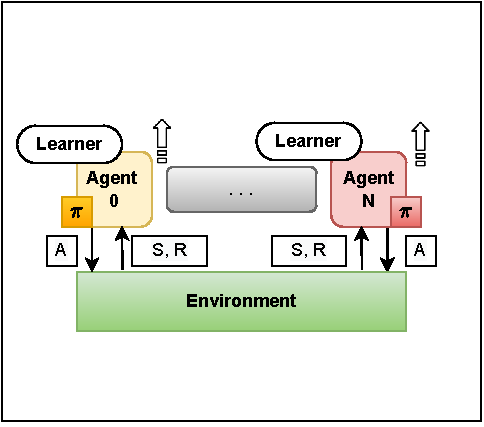
\includegraphics[width=\textwidth]{{img/dtde.pdf}}
    \caption{Independent learners and controllers}
  \end{subfigure}
  \hfill
  \begin{subfigure}[t]{0.49\textwidth}
    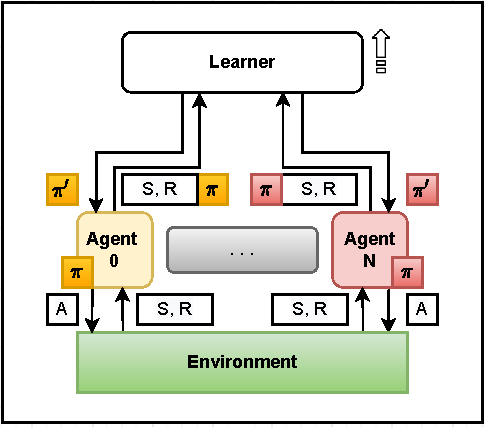
\includegraphics[width=\textwidth]{img/ctde.pdf}
    \caption{Centralized learner and Decentralized controllers}
  \end{subfigure}
  \caption{Two learning schemas in \ac{marl}. In independent learners, each agent refines their policy through local experience. In \ac{ctde} instead, a global learner is used to find local policies.}
  \label{coordination2022:fig:cdte}
\end{figure} For now, I had removed that figure. I think that it does not give so much info @RC what do you think?
In \ac{ctde}, a central agent performs the learning process and generates distributed controllers, one for each agent. 
%
\ac{ctde} is typically applied in offline learning through the use of simulations. 
%
This way, it is possible to leverage global information at simulation time, but then the controllers are completely independent of this central authority.  
%
So, when the learner finds a good policy, it can be removed from the system. 

Although \ac{ctde} allows \ac{rl} to be used in environments with many agents, the learner must consider a large population of agents at simulation time, leading to sample inefficient algorithms.
%
A solution to this problem in similar \acp{cas} (e.g. swarm robotics~\cite{DBLP:conf/atal/SosicKZK17}) is to add another constraint, namely the agents' homogeneous and cooperative behaviour~\cite{DBLP:journals/aamas/PanaitL05}. 
%
With this assumption, the learner only has to find a single strategy that applies to the whole system.%, which reduces complexity and the non-stationary.
%
%Obviously, this also reduces the solution space, but in \acp{cas} the condition of homogeneity is acceptable because simple controllers can still produce complex collective behaviour as observed in nature.

\section{Reinforcement Learning-based Aggregate Computing}\label{coordination2022:s:contrib}
%\meta{
%  \begin{itemize}
%    \item clarify the motivation
%    \item integration perspective: architectural-level (message delivery, round frequency, opportunistic deployment)
%    \item integration perspective: building block optimization (why, current solution)
%  \end{itemize}
%}
\end{comment}
\section{On Integrating Machine Learning and Aggregate Computing}

As anticipated in \Cref{chap:macro-programming}, the behaviour of an aggregate system depends on the interplay of three main ingredients:
 (i) the aggregate program, expressing conceptually the global behaviour of the entire system, and concretely the local behaviour of each individual node in terms of local processing and data exchange with neighbours; and 
 (ii) the aggregate execution model, promoting a certain dynamics of the system in terms of topology management (e.g., via neighbour discovery), execution of rounds, scheduling of communications; and
 (iii) the environment dynamics.
%
While the latter cannot be controlled, 
 the importance of the first element is reflected by research
 on the design of novel algorithms (cf.~\cite{DBLP:journals/jlap/ViroliBDACP19,DBLP:conf/saso/AudritoCDV17}),
 while the second element is studied 
 w.r.t. the possibility of tuning and adaptivity 
 according to 
 available technology and infrastructure 
 or the dynamics of the environment. %(e.g. reacting to a phenomenon that changes quickly requires increasing the execution frequency---cf.~\cite{danilo2021lmcs}).
%
Since tuning programs or execution details to specific environments
 or adapting those to changing environments
 can be burdensome,
 it makes sense to consider the use of Machine Learning techniques
 to let a system \emph{learn} effective strategies for unfolding collective adaptive behaviour.
%

\section{Aggregate Programs Improvement through \ac{rl}}
%!TeX root = paper22-coord-ac-rl.tex

\begin{figure}[t]
  \centering
  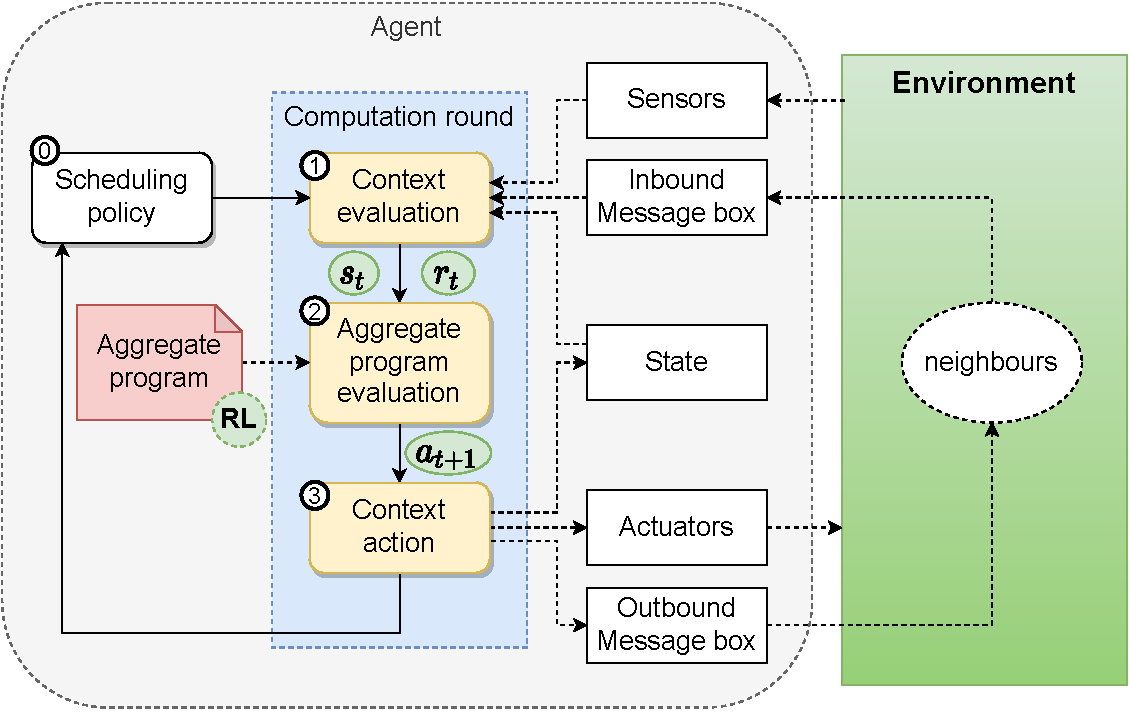
\includegraphics[width=0.9\textwidth]{papers/coordination2022/img/aggregate-agent-control-architecture.pdf}
  \caption{Integration of \ac{rl} within the \ac{ac} control architecture~\cite{DBLP:journals/jsan/CasadeiAV21}. 
  %
  The \ac{rl} state and reward concepts build upon the context, given by environment and neighbour data. 
  %
  The designer configures action points where learning can improve the aggregate computation. 
  %
  The actions selected by the learned policies will then affect the environment (via actuators) and neighbours (via outbound messages).}
  \label{fig:ac-and-rl}
\end{figure}

In this work, we focus on \emph{improving aggregate programs}
 by learning effective local actions
 within a given algorithmic schema---an approach similar to the \emph{sketching} technique for program synthesis~\cite{solar2008program-synthesis-sketching}.
% \meta{TODO: explain why RL and not other ML techniques}.
As a learning framework,
 we use \ac{rl} as 
 we deal with systems of agents 
 performing ongoing activities 
 by interacting with one another and the environment. 
 %it makes it possible to exploit learning even in cases where we do not know the optimal result for a certain program, but we can only evaluate its performance under certain circumstances (either with simulations or directly in concrete systems). 
% 
From a local viewpoint, an \ac{ac} device is an agent acting based on the local context it perceives (sensor readings, device state, and messages from neighbours), and this matches the \ac{rl} execution model very well.

So, our long-term goal is to integrate \ac{rl} into the \ac{ac} ``stack'' (i.e., across the platform, language, and library levels) to improve the collective behaviour defined by \scafi{} aggregate programs in terms of \emph{efficiency} (i.e., reducing the resource usage maintaining the same functional interface), \emph{efficacy} (i.e., synthesizing more stable and faster converging behaviours) and \emph{adaptability} (i.e., the same program works against different environments).
%

As a first contribution, summarized in \Cref{coordination2022:fig:ac-and-rl}, in this work we integrate \ac{rl} within the \ac{ac} control architecture in order to support learning of good collective behaviour sketched by a given aggregate program.
%
Specifically, we focus on improving \ac{ac} building blocks (such as the gradient algorithm covered in \Cref{coordination2022:sec:gradient}) through learning, leading toward a so-called \emph{Reinforcement Learning-based Aggregate Computing}. 
%
Learning, thus, does not replace the \ac{ac} methodology for defining the programs, but it is best understood as a technique that supports and improves the \ac{ac} algorithm design process. %, especially for handling critical situations (e.g. unpredictable environment dynamics, opportunistic deployments, etc.).
%
%In such a new paradigm, we combine the advantages of \ac{ac}, hence compositionality and self-organisation, with those of \ac{rl}, such as goal-oriented and adaptable behaviours.

%\meta{RC: non riusciamo a far vedere un'immagine dove la figura di RL si integra con la control architecture di AC (tipo immagine in paper MDPI-JSAN)? }
%However, we also think that learning could improve execution platform aspects. \meta{subsection? or paragraph? Or it is ok as it is?}
%%
%Indeed, \ac{ac} abstracts over various infrastructural matters, such as neighbourhood discovery, message delivery, round scheduling and aggregate programs deployment. 
%%
%These aspects, though, are essential to accomplish some \ac{qos}. Therefore, learning will be an inherent technique to improve \ac{qos} maintaining the same aggregate program.
%
%Recent works already explore the idea of improving QoS without changing the system-wide program. 
%%
%In the \ac{ac} context, \emph{distributed schedulers} define a way to program the round scheduling in order to reduce the system-wide power consumption. 
%%
%The \emph{pulverisation} approach instead describes the main independently deployable components for supporting a collective computation. 
%%
%In this way, the same program is easily deployable in different IT infrastructures -- a so-called \emph{fluid} computation.
%
%Thus, learning algorithms could be combined with the above ideas to let the system self-adapt directly through raw experience.

\section{Building blocks Refinement}\label{coordination2022:s:learning-gradient}
%\meta{@GA: this may became a subsection of Reinforcement Learning-based AC?}
%\meta{
%  \begin{itemize}
%    \item State-of-the-art solution -- heuristic strategy to solve some problems
%    \item Intuition: RL used to learn these policies by experience
%    \item devise the learning settings (partial observable env, local neighbourhood, local action)
%    \item devise the design process of a learning block (state, action, reward definition)
%  \end{itemize}
%}

A major advantage of \ac{ac} as a programming model is its \emph{compositionality}: complex collective behaviours (e.g., the maintenance of a multi-hop connectivity channel) can be expressed through a combination of building blocks capturing simpler collective behaviours (e.g., gradients).
%
Since building blocks are fundamental bricks of behaviour that often recur in programs, 
 their bad and good qualities (cf., convergence speed, stability, etc.) tend to amplify and affect behaviours that depend on them.
%
%Even if AC is independent of IT infrastructure, several behaviours tend to have a long self-stabilisation time in some deployments w.r.t the idealised convergence time, leading to non-stable and unpredictable aggregate programs.
%
Therefore, research tends to investigate refined variants of building blocks that provide the same functionality but are more effective or efficient under specific assumptions or contexts (e.g., high mobility, situations where stability is more important than precision, etc.)~\cite{DBLP:conf/saso/AudritoCDV17,DBLP:journals/cee/AudritoCDPV21}.
%
With a library of algorithms, the designer can choose the best combination of building blocks that are well-fitted for a given environment, and even substitute a building block with a variant implementation without substantially affecting the application logic.
%\meta{@GA to @All, in sec 4.1 I show a gradient block with opt. Probably here we need to show a general structure? With images? }
In general, a building block can be seen as a black box (function) that takes a set of input fields (e.g. metric, perception fields, constant fields, etc.) and yields an output field. 
%
To increase its flexibility, such a function could leverage a \emph{refinement policy} able to affect the behaviour of the building block over time or in a certain situation. 
%
This policy could be a feedback loop, hysteresis, or custom logic to solve a specific problem.
%
We aim at structuring the learning of refinement policies through \ac{rl}~\cite{DBLP:conf/acsos/Aguzzi21}.
%
Our idea is that it should not be the designer who codes a particular block to be used, but that it is the learning algorithm that understands, given a global policy to be optimized following a utility function, what actions need to be activated.
% to optimise the collective good of the system.

%!TeX root = paper22-coord-ac-rl.tex
\begin{figure}[t]
  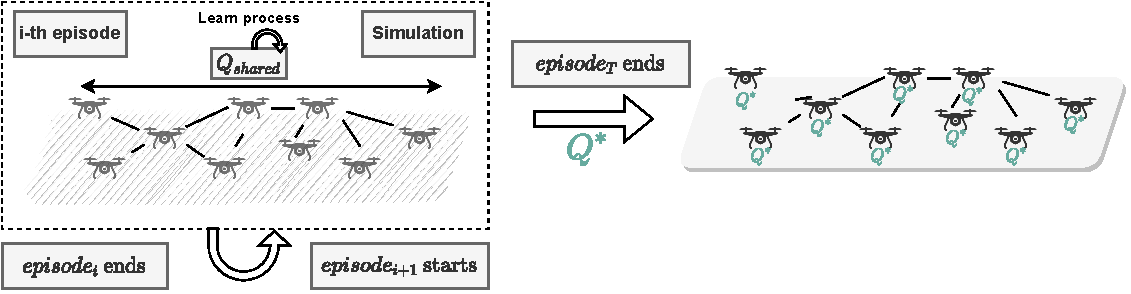
\includegraphics[width=\textwidth]{papers/coordination2022/img/algorithm-learning.pdf}
  \caption[Reinforcement Learning schema used in program synthesis simulations]{
  Reinforcement Learning schema used in our simulations.
  The learning algorithm is applied at simulation time (for $T$ episodes) improving a shared $Q$ table. 
  %
  At the deployment time then, the agents exploit a local copy of the optimal $Q^*$ table found by learning.}
  \label{fig:learning-scheme}
\end{figure}
However, using Machine Learning to improve \ac{ac} programs exposes several non-trivial challenges:
\begin{itemize}
  \item \emph{scale-free behaviours}: the learned policy should work in small networks as well as in large networks as fostered by the \ac{ac} abstractions;
  %% not discussed, remove for now
  %\item the local agent state depends upon a \emph{variable neighbourhood}: the aggregate computing programs reach collective computation through local agents interactions that are not fixed;
  \item the state typically depends on \emph{continuous} value as computational fields are often associated with continuous data (e.g. temperature or distance fields);
  \item \emph{multi-agent credit assignment problem}: 
   it is not easy to adequately reward and credit local actions for their contribution to the eventual convergence to
   the ``target'' field denoting the desired, emergent, collective result.
   %the utility function could be computed by means of the collective computational fields, hence should be difficult to weigh a local agent action. 
\end{itemize}
%
The \ac{ac} system model is based on \emph{cooperative} and \emph{homogeneous} behaviour. 
%
Indeed, when a node participates in an aggregate system, it has to execute an aggregate program shared within the whole system, which yields different outcomes according to the contexts on which it gets evaluated. 
%
This leads to handling homogeneous \ac{marl}, hence our goal will be to find one policy for the entire ensemble, partially solving the scale-free behaviour problem, since the learned policy will not depend on the system's size.

The continuous and variable state problems are typically tackled using Deep Learning to learn the right state representation for a given problem~\cite{DBLP:journals/corr/abs-1806-08894}. %and Graph Neural Networks (to regulate variable-size inputs). 
%
In this case, instead, we used a handcraft feature engineering process since we are more interested in devising a general design process.

Concerning the \emph{multi-agent credit assignment problem}, we decided to use offline learning 
%based on simulation and then the policy is deployed in a concrete system 
in a typical \ac{ctde} setting (\Cref{coordination2022:fig:learning-scheme}).
%
This way, we assess the influence of an individual in comparison to the entire system, which cannot be done in online learning due to the difficulty of achieving global snapshots of the system in a reasonable time.


\section{Learning Schema} 

The learning algorithm is seen as a state ($s_t$) evolution function in which the nodes try to apply a correction factor (\lstinline|update|) following a policy ($\pi^Q_{target}$ or $\pi^Q_{behavioral}$) refined by learning.
%
The state is built from a neighbourhood field of the building block generic output ($o_t$) passed as input.
%
\Cref{coordination2022:lst:general-schema} exemplifies the general program structure used to combine \ac{rl} with \ac{ac} for improving building blocks.
%
The branching operator (\lstinline|branch|) on \lstinline|learn| condition makes it possible to use the \ac{ctde} schema since when the \lstinline|learn| is \lstinline|false| there is no need for a central entity (\lstinline|simulation|).
%
The Q table is gathered using \lstinline|sense|, a \scafi{} operator used to query sensors and collect data from them. 
%
At simulation time, Q is a shared object, but at runtime each agent owns a local table.
%
%!TeX root = paper22-coord-ac-rl.tex

\begin{lstlisting}[
  mathescape,
  %float=tp,
  floatplacement=tbp,
  frame=single,
  label={coordination2022:lst:general-schema},
  caption={
    ScaFi-like pseudocode description (implemented in the simulation) for value-based \ac{rl} algorithm applied \ac{ac}.
    %
    \texttt{state}, \texttt{update}, \texttt{reward} are block specific. 
    %The learn branch use \texttt{simulation}, a global object in which agents access to a shared Q.
  },
  captionpos=b
]
def optBlock($o_{t-1}$) { // learning as a field that evolves in time
  rep(($s_0, a_0$, $o_0$)) { // $s_0$, $a_0$ context dependent 
    case ($s_{t-1}, a_{t-1}$, _) => {
      val Q = sense("Q") // global during training, local during execution
      val $o_{t}$ = update($o_{t-1}$, $a_{t-1}$) // local action
      // state from the neighbourhood field program output
      val $s_{t}$ = state(nbr($o_{t}$))
      val $a_{t}$ = branch(learn) { // actions depends on learn condition
        val $r_{t-1}$ = reward($o_{t}$, simulation) // simulation is a global object
        simulation.updateQ(Q, $s_{t-1}$, $a_{t-1}$, $r_{t-1}$, $s_{t}$) // Q update
        $\sim$ $\pi_{behavioural}^Q$($s_{t}$) // sample from a probabilistic distribution
      } {
        $\pi_{target}^Q$($s_t$) // greedy policy, no sampling is needed
      }
    }
    ($s_{t}$, $a_{t}$, $o_{t}$) 
  }._3 // select the output from the tuple
}
  \end{lstlisting}
  %\caption{\scafi{}-like pseudocode description for value-based \ac{rl} algorithm applied \ac{ac}. \texttt{state}, \texttt{update}, \texttt{reward} are block specific. The learn branch use \texttt{simulation}, a global object in which agents access to a shared Q. 
  %$\sim$ stands for sampling a value from a probabilistic distribution.}
  %\label{lst:general-schema}
%\end{figure}
%
Finally, the produced $o_{t}$ is returned to the caller.

In this case, we encoded the learning process with \ac{ac} itself. 
%
Though we could have extracted the learning process from the \ac{ac} program, %producing a policy usable in \ac{ac},
 we took this decision because: 
  (i) it allows us to extend learning by exploiting neighbourhood Q table fields -- so we can think of doing non-homogeneous learning in different areas of the system;
  (ii) the scheme for taking state and choosing actions is the same as the one we would need for learning, so the only difference is in the branch; and
  (iii) it can simply be extended to online learning.
%
%In the next section, we describe an incarnation of this algorithm applied to the gradient block.

\section{Reinforcement Learning-based gradient block}
%\meta{
%  \begin{itemize}
%    \item describe the block G -- why it is important, for what is used 
%    \item G problems -- stable results, count-to-infinity, speed bias
%    \item try to describe a general G block that accept an optimisation/correction strategy
%    \item define the Reinforcement Learning as an optimisation block
%  \end{itemize}
%}

%\meta{@GA to @All: another way to generalise G?}
The gradient block could be generalized as follows:
\begin{lstlisting}
def gradientOpt(source, metric, opt) {
  rep(infinity) { g => mux(source) { 0 } { opt(g, metric) } }
}
\end{lstlisting}
where \lstinline|opt| is a function that determines how to evolve the gradient based on the field of current gradient values \lstinline|g| and current \lstinline|metric| (estimation of distances to neighbour). 
%In this way, the correction factor applied to the gradient could be composed, creating a gradient block that handles several scenarios.
In this article, we consider \lstinline|opt| as a \emph{hole} that a \ac{rl} algorithm will fill through raw experience
 with actions aiming at incrementally constructing a gradient field, hopefully mitigating the \emph{rising-value} issue (cf. \Cref{coordination2022:sec:gradient}).
%
To frame our learning problem, we adopt the above-described general schema (\Cref{coordination2022:fig:learning-scheme}). The state and action functions are inspired by the CRF algorithm.
%
The \lstinline|state| function must hold enough information to know when agents should speed up the local rising of values.
%
In this case, we encode the state as the difference between the output perceived by a node and the minimum and maximum gradient received by its neighbours: $s_t = (|min_t - o_t|, |max_t - o_t|)$. 
%
These data have to be discretized; otherwise, the search space would be too big and the solution could suffer from overfitting. 
%
The discretization is ruled by two variables, $maxBound$ and $buckets$. 
%
The former constrains the output to be between $ - radius * maxBound$ and $ radius * maxBound $ (where $radius$ is the maximum communication range of the nodes). 
%
The values outside that range will be considered as the same state.
%
The $buckets$ variable rules the division count of the given range. 
Finally, we stack two time steps in order to encode history inside the agent state:
$h_t = [(s_{t - 1}, s_t)]$. $h_t$ is used as the state function for our \ac{rl} algorithm.
Hence, the cardinality of the state space of $|s_t| * |s_t| = buckets^4$. 
%
The action space is divided into two action types: \texttt{ConsiderNeighbourhood} is the action that will produce the classic gradient evaluation, while 
 \texttt{Ignore(velocity)} ignores the neighbour data and increases the gradient at a given \texttt{velocity}. So, the \texttt{update} function is defined as:
\begin{lstlisting}[mathescape]
def update($o_{t-1}$, $a_{t-1}$, metric) = // $o_{t-1}$ is the previous gradient output
  val $g_{classic}$ = minHoodPlus(nbr($o_{t-1}$) + metric())
  match $a_{t-1}$ // scala-like pattern matching
    case ConsiderNeighbourhood => $g_{classic}$
    case Ignore(velocity) => $o_t$ + velocity * deltaTime() 
\end{lstlisting}
%
Finally, the \texttt{reward} function is described as follows: 
\begin{lstlisting}[mathescape]
def reward($o_t$, simulation) {
  if($o_t$ - simulation.rightValueFor(mid()) $\sim$= 0) { 0 } { -1 }
}
\end{lstlisting}
where \lstinline|mid| returns the field of node identifiers. 
%%
The idea is to push the nodes to produce an output that is very close to the ideal, correct gradient value as provided by an oracle (\lstinline|simulation.rightValuefor()|).
%%
When this is the case, we provide a value equals to $0$;
instead, when the value is different from the expected one, 
 we provide a small negative reward, $-1$, in order to push the nodes to quickly seek the situation where the actual and ideal value match.

\section{Evaluation}\label{coordination2022:s:eval}

\begin{table}[t]
  \centering
  \begin{tabular}{|c|c|}
    \hline
    Name &  Values \\ \hline
    $(\gamma)$ & [0.4 -- 0.7 -- 0.9] \\  \hline
    $(\epsilon_0, \theta)$ & [(0.5,200) -- (0.01,1000) -- (0.05,400) -- (0.02,500)] \\ \hline
    $(\beta, \alpha)$ & [(0.5,0.01) -- (0.5,0.1) -- (0.3,0.05) -- (0.2,0.03) -- (0.1,0.01)]
    \\  \hline
    (buckets, maxBound) & [(16,4) -- (32,4) -- (64,4)]\\ \hline
  \end{tabular}
  \caption{Summary of the simulation variables. 
  %
  A simulation is identified by a quadruple $(i, j, k, l)$ of indexes for each variable. 
  %
  %So simulation 0000 is the one with $\gamma = 0.4, \epsilon_0 = 0.5, \theta = 200, \beta = 0.5, \alpha = 0.01, buckets = 16,  maxBound = 4$.
  }
  \label{coordination2022:table:parameters}
\end{table}

To evaluate our approach, we run a set of simulated experiments and verify that an aggregate system
 can successfully learn an improved way to compute a gradient field (cf. the gradient block described in \Cref{coordination2022:sec:gradient}).
%
To this purpose, we adopt Alchemist~\cite{DBLP:journals/jos/PianiniMV13},
 a flexible simulator 
 for pervasive and networked systems
 that comes with a support for aggregate systems 
 programmed with \scafi{}~\cite{DBLP:conf/isola/CasadeiVAD20}. 
%
The source code, data, and instructions for running the experiments have been made fully available at a public repository\footnote{\url{https://github.com/cric96/experiment-2022-coordination}}, to promote reproducibility of results.

\subsection{Simulation setup}

The simulated system consists of $N$ devices deployed in a grid. 
%
We use two kinds of grid-like environments. 
%
They both have the same width (\SI{200}{\metre}) and distance between nodes (\SI{5}{\metre}), but they differ in the row count. 
%
In one case, only one row exists (so the nodes are placed in a line). 
%
In the other case, there are five rows. 
%
The total number ($N$) of agents is then defined as $ 200 / 5 * rows $. 
%
So in the first case, we have a total of 40 agents, in the second case we have 200 agents. 
%
Each node asynchronously fires the round evaluation at \SI{1}{\hertz}.
%
The leftmost and the rightmost agents are marked as source nodes. 
%
Each simulated episode lasts \SI{85}{\second} ($T$).
%
For simulating the slow rising problem, we drop the left source at \SI{35}{\second} ($C_s$), and so the left part of the system starts to rise until eventually stabilizing to the correct computational field.
%
An entire simulation lasts $N_E = 1200$ episodes, in which in the first $N_L = 1000$ the system uses \ac{rl} to improve a shared Q table, and then in the last $N_T = 200$, the system deploys the Q table found in each agent. 
%
In these last runs, the agents act following the greedy policy.

As learning algorithm, we used Hysteretic Q-Learning (cf. \Cref{coordination2022:s:background:rl}). %, since it tackles environments stochasticity.
%
As behavioural policy, we use an $\epsilon$-greedy with an exponential decay to balance the exploration-exploitation.
%
We make this choice because without using the decay the policy found tends to be not optimized (i.e. the exploration is preferred w.r.t exploitation).
%
At each episode $i$, the $\epsilon$ value is updated as $\epsilon_i = \epsilon_0 \cdot e^{{i} / \theta}$.

Several variables are used, summarized in \Cref{coordination2022:table:parameters}, so we perform a grid search to find the optimal combination.
%
To evaluate a particular configuration, we verified the total error performed in the last $N_T$ episodes.
%
This is calculated from the error performed by each node $i$ at each time step $t$:
\begin{equation}
error_i^{t} = |gradient_i^{t} - simulated_i^t|
\end{equation}
Then for each time step $t$, we evaluate the average system error as:
\begin{equation}
error_{t} = \frac{1}{n}\sum_{i = 0}^N error_i^t
\end{equation}
And finally, the error of each episode is evaluated as:
\begin{equation}
error_{episode} = \sum_{t = 0}^T error_{t}
\end{equation}
We choose the configuration by observing the box plots (\Cref{coordination2022:subfig:boxplot}) and taking the lowest average error in the last $N_T$ episodes.

%!TeX root = thesis-main.tex
\newcommand{\figfactor}{0.45}
\begin{figure}[t!]
  \bigskip
  \begin{subfigure}[t]{\figfactor\textwidth}
    \centering
    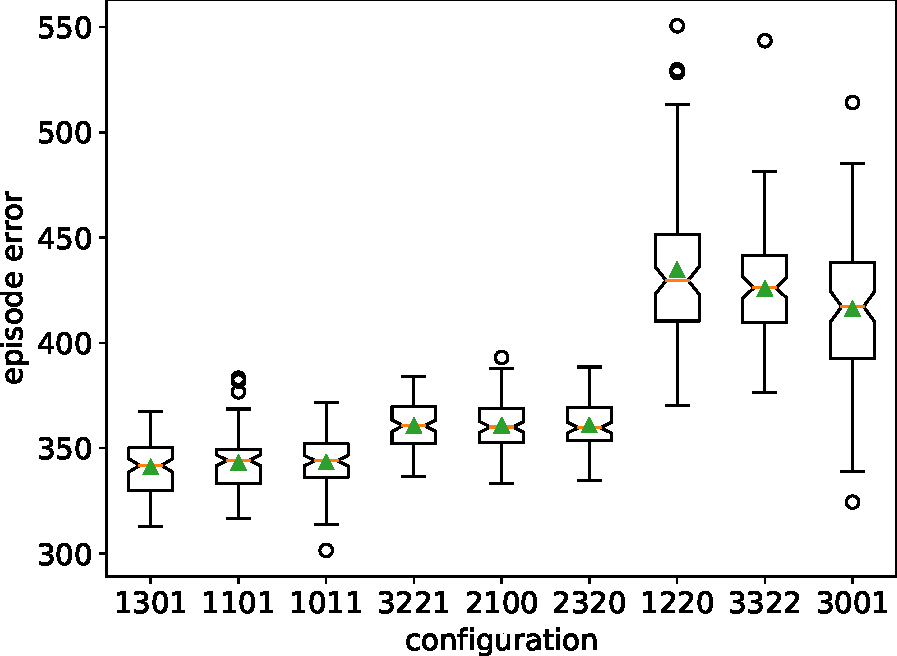
\includegraphics[width=\textwidth]{papers/coordination2022/img/box-all.pdf}
    \caption{Box plots of last $G_s$ episode.}
    \label{coordination2022:subfig:boxplot}
  \end{subfigure}  
  \hfill
  \begin{subfigure}[t]{\figfactor\textwidth}
    \centering
    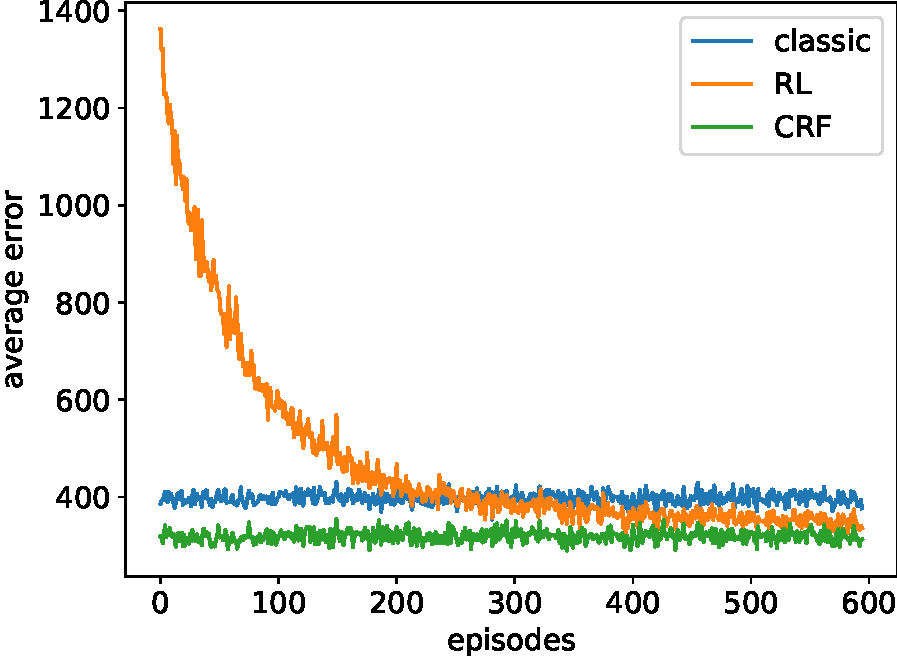
\includegraphics[width=\textwidth]{papers/coordination2022/img/mean-error-left.pdf}
    \caption{Learning progress of the best result.}
    \label{coordination2022:subfig:mean-error-over-episode}
  \end{subfigure}
  \bigskip
  
  \begin{subfigure}[t]{\figfactor\textwidth}
    \centering
    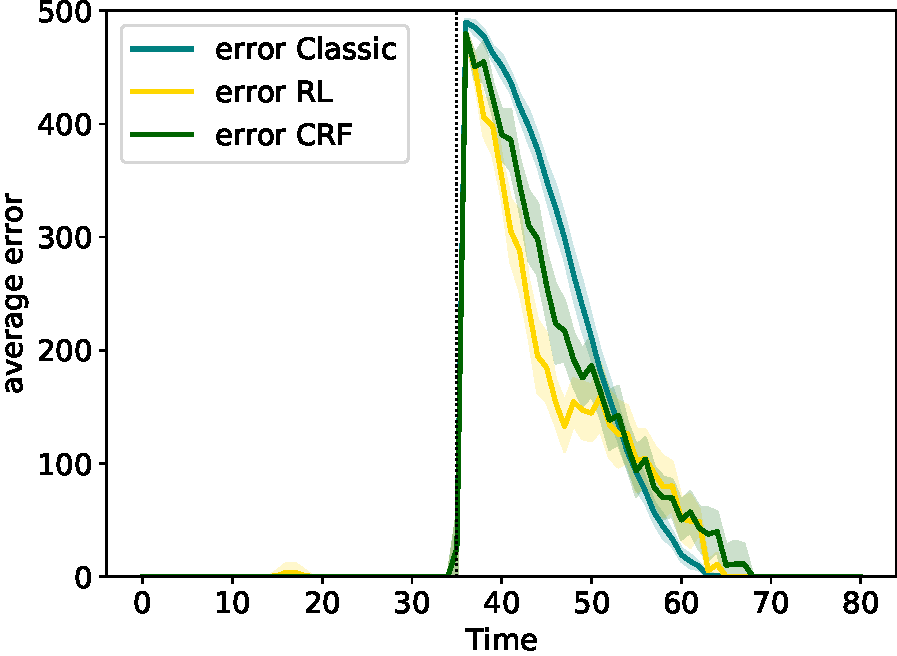
\includegraphics[width=\textwidth]{papers/coordination2022/img/error-few-nodes.pdf}
    \caption{Error evolution with 40 agents}
    \label{coordination2022:subfig:error-few}
  \end{subfigure}
  \hfill
  \begin{subfigure}[t]{\figfactor\textwidth}
    \centering
    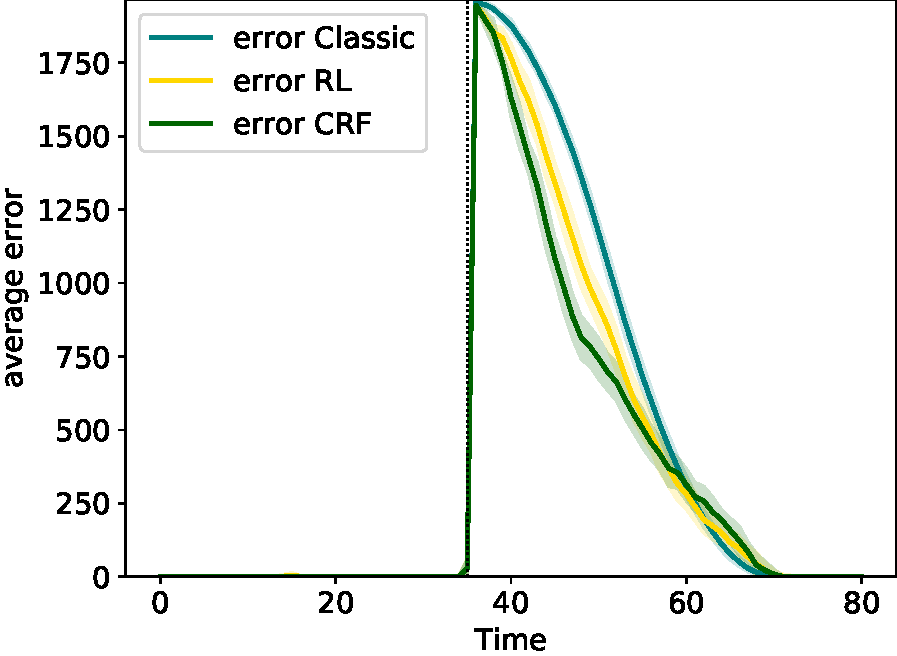
\includegraphics[width=\textwidth]{papers/coordination2022/img/error-many-nodes.pdf}
    \caption{Error evolution with 200 agents}
    \label{coordination2022:subfig:error-many}
  \end{subfigure}
  \bigskip
  
  \begin{subfigure}[t]{\figfactor\textwidth}
    \centering
    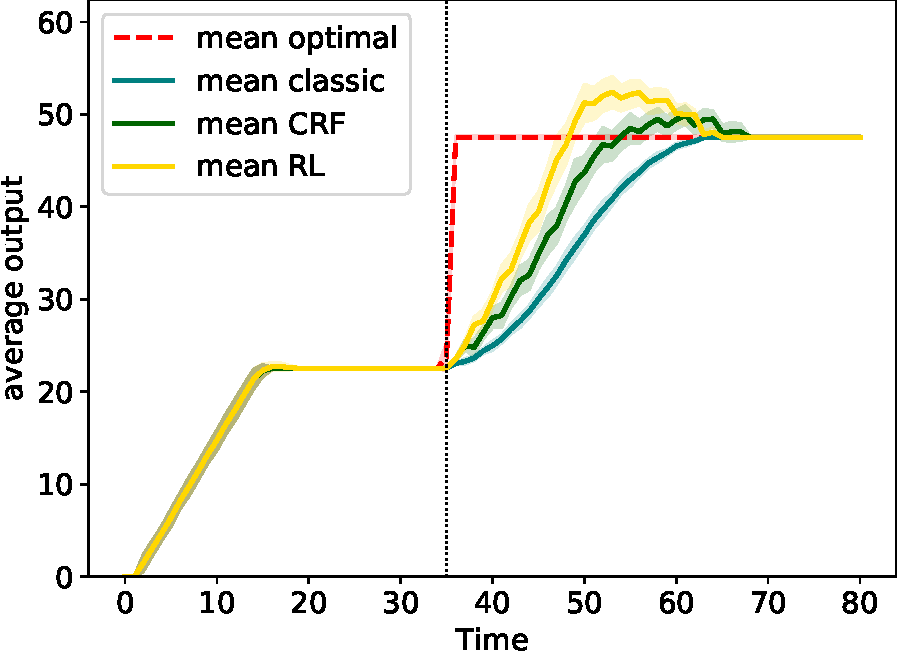
\includegraphics[width=\textwidth]{papers/coordination2022/img/output-few-nodes.pdf}
    \caption{Output evolution with 40 agents}
    \label{coordination2022:subfig:output-few}
  \end{subfigure}
  \hfill
  \begin{subfigure}[t]{\figfactor\textwidth}
    \centering
    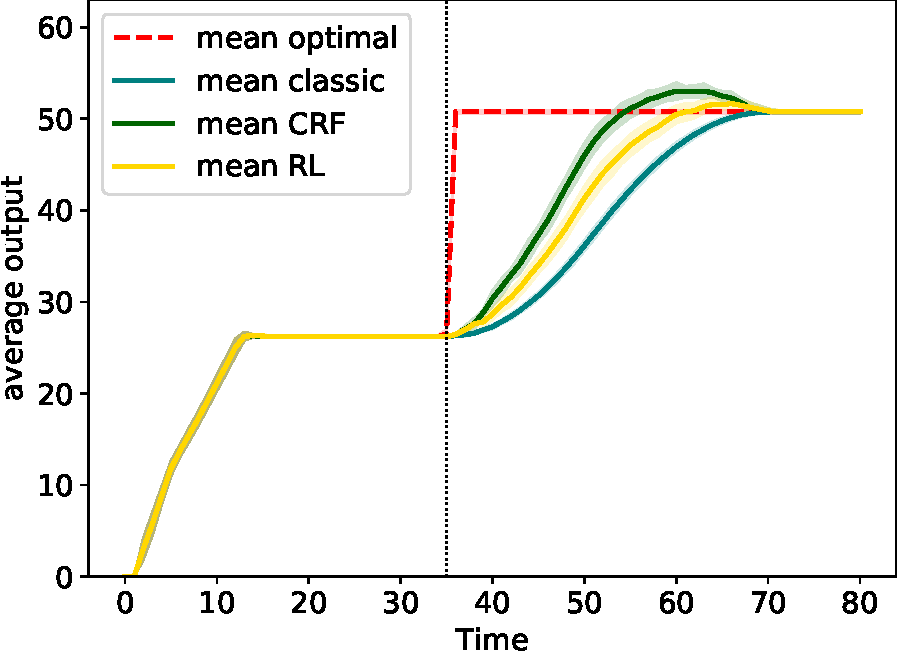
\includegraphics[width=\textwidth]{papers/coordination2022/img/output-many-nodes.pdf}
    \caption{Output evolution with 200 agents}
    \label{coordination2022:subfig:output-many}
  \end{subfigure}
  \caption{Performance of our \ac{rl}-based gradient algorithm with \lstinline|velocity| = 20.
  }
  \label{coordination2022:fig:eval}
\end{figure}
\subsection{Results and Discussion}

\Cref{coordination2022:fig:eval} shows the performance of our \acl{rl}-based gradient algorithm.
%
\Cref{coordination2022:subfig:boxplot} was used to choose which configuration was the best.
%
\Cref{coordination2022:subfig:mean-error-over-episode} shows the error trend as the episodes change. 
%
The second row shows the trend of the mean error over the last $N_T$ episodes. 
%
The coloured area under the curve defines the standard deviation. 
%
The dashed vertical line is the time at which the source change occurs. 
%
Finally, the last row shows the average output of the various algorithms. 
%
In the following we discuss the result reached with the best configuration, that has $\gamma = 0.9$, $\epsilon_0 = 0.5$, $\theta = 200)$, $\alpha=0.3$ and $\beta=0.05$. 

Our goal was to create a solution that outperforms the classic gradient against the rising-value problem.
%
In fact, the system eventually learns how to speed up the gradient rising: observing the \Cref{coordination2022:subfig:mean-error-over-episode} the $error_{episode}$ of the new algorithm is lower than the error produced by the standard solution. 
%
In particular, this means that the agents learn the moment when they should ignore their neighbourhood and increase the output with a certain velocity (i.e. using the \lstinline|Ignore| action).

This intuition is enforced by \Cref{coordination2022:subfig:error-few,coordination2022:subfig:error-many,coordination2022:subfig:output-few,coordination2022:subfig:output-many}.
% 
In particular, in \Cref{coordination2022:subfig:error-few,coordination2022:subfig:output-few} the behaviour is more evident due to the reduced number of agents: when the error is maximized (due to the source that disappears), the error decreased faster than the naive gradient (and, consequently, the output is faster growing).
%
Furthermore, we can also observe that the overall algorithm behaviour is comparable with the CRF handcrafted solution for the rising problem. 
%
Indeed, both have a phase of speed up followed by another phase of overestimation (i.e. the system-wide output is greater than the true gradient field output) that eventually brings the system to slowly reaches the correct value.
%
Moreover, not only the \ac{rl}-based solution has similar behaviour to CRF, but also it has comparable performance -- it means that the aggregate reaches a near-optimal policy with these state-action-reward settings.

We want also to underline that the policy learned is \emph{one} and shared with the whole system.  
%
Thereby, the policy can be easily scaled in deployments with different node counts. 
%
In this case, the \emph{same} function outperforms our baseline in a system with different nodes and deployment configurations. 
%
%The current issue is, however, that we cannot prove that this policy works with any possible deployment: this needs to be evaluated in future work.

Finally, we want to stress that the nodes do not fire synchronously, and thus there is not any kind of global and shared clock: any node round evaluation order reaches the same behaviour in our test deployments. 
%
This, again, makes it possible to use the same policy in different scenarios due to the unknown local aggregate programs evaluation order.

\section{Wrap up}\label{coordination2022:s:conc}

This chapter discusses the integration of \acl{ac} -- a programming approach for \aclp{cas} -- and \acl{rl}, with the goal of fostering the design of collective adaptive behaviour.
% 
In particular, we propose to use \ac{rl} as a means to improve building block \ac{ac} algorithms. %- in a similar way to what is done in program synthesis. 
%
Our approach is applied to improving the gradient algorithm, one of the key \ac{ac} algorithms, where learning is performed through Hysteretic Q-Learning.
%
We evaluate the approach through synthetic experiments comparing the reactivity of different gradient algorithms in dealing with the rising value problem.

%\printbibliography